\documentclass{article}


% Formatting
\usepackage[utf8]{inputenc}
\usepackage[margin=1in]{geometry}
\usepackage[titletoc,title]{appendix}

% Math
% https://www.overleaf.com/learn/latex/Mathematical_expressions
% https://en.wikibooks.org/wiki/LaTeX/Mathematics
\usepackage{amsmath,amsfonts,amssymb,mathtools}

% Images
% https://www.overleaf.com/learn/latex/Inserting_Images
% https://en.wikibooks.org/wiki/LaTeX/Floats,_Figures_and_Captions
\usepackage{graphicx,float}

% Tables
% https://www.overleaf.com/learn/latex/Tables
% https://en.wikibooks.org/wiki/LaTeX/Tables

% Algorithms
% https://www.overleaf.com/learn/latex/algorithms
% https://en.wikibooks.org/wiki/LaTeX/Algorithms
\usepackage[ruled,vlined]{algorithm2e}
\usepackage{algorithmic}

% Code syntax highlighting
% https://www.overleaf.com/learn/latex/Code_Highlighting_with_minted
\usepackage{minted}
\usemintedstyle{borland}

% References
% https://www.overleaf.com/learn/latex/Bibliography_management_in_LaTeX
% https://en.wikibooks.org/wiki/LaTeX/Bibliography_Management
\usepackage{biblatex}
\usepackage{subfig}
\usepackage{movie15}
\addbibresource{references.bib}

% Title content
\title{Math 3550 - Fourier Series and the Wave Equation}
\author{Ammaar Firozi}
\date{May 5, 2021}

\begin{document}

\maketitle

% Abstract
\begin{abstract}
This paper initially covers the wave equation and derives its solution. From there, several orthonormality identities of the wave equation are proven, and the requirements of the wave equation's coefficients are determined. Then, several functions' Fourier series are computed and MATLAB is used for error comparison. Finally, Fourier series are used to determine the 1-D wave equation for a string of fixed length. 
\end{abstract}

% Introduction and Overview
\section{Introduction and Overview}

The goal of Fourier series is to express complicated periodic signals as linear combinations of sines and cosines or, in other words, to express these periodic signals as the superposition of a variety of waves. 

% Example Subsection
\subsection{Periodic Functions}
Suppose that $\ f(t)$ is periodic with period $\ T$, i.e., $\
f(t)=f(t+nT), t \in \mathbb{R}, n \in \mathbb{Z}$ . On the interval $\ [ \, 0, T ] \,$, $\ f(t)$ will produce the same function output on any other interval of length $\ T$. Suppose a wave was generated on the interval$\ [ \, 0, T ] \,$,  the period of the wave, $\ T_{wave}$, must follow the statement: $\ T_{wave} |  T$  . Following this, the circular frequency of such a wave would be $\ \omega_{wave}=\frac{2\pi}{T_{wave}}=\frac{2\pi n}{T}$. Collecting all sines and cosines with the mentioned frequencies with a constant function $\ f(t) $ can be written as follows:
\begin{equation}
    f(t)=a_{0}+\sum_{n=1}^{\infty} [a_{n} \cos(\frac{2\pi nt}{T})+b_{n} \sin(\frac{2\pi nt}{T})], 0 \leq t \leq T
\end{equation}
It should be noted that the convergence of (1) is not guaranteed for all $\ a_n$ and $\ b_n$ values. However, explaining why is beyond the scope of this paper, and for the purposes of this paper, there should be no issues of convergence. However, the coefficients $\ a_n$ and $\ b_n$ are still required to represent the function $\ f(t), 0 \leq t \leq T$. These proper coefficients will be discussed further later on in the paper.

The Fourier series can be related to differential equations. For example, consider the general second order differential equation with constant coefficients

\begin{equation*}
	x''(t) + px'(t)+qx(t)=f(t).
\end{equation*}
From this, we can define a linear differential operator $T$, such that $T$[$x$] $=x''+px'+qx$. From the operator's linearity, the principle of superposition leads to the following relationship
$T(x_{1}) = f_{1}$ and   $T(x_{2})=f_{2}$  $\implies T(x_1+x_2)=f_1+f_2$.

From this result, the Fourier series can be used. Clearly, solving the non-homogeneous differential equation above, where $f$ represents an arbitrary periodic function, can be done by replacing $f$ by its Fourier series and solving the differential equations
\begin{equation*}
	x''(t)+px'(t)+qx(t)=a_{n}\cos(\frac{2\pi nt}{T})+b_{n}\sin(\frac{2\pi nt}{T})
\end{equation*}for $n \in \mathbb{Z}^{nonneg}$

\subsection{The Wave Equation}
Consider a vibrating string of length $l$ oriented on the x-axis such that its left end is at $x=0$. Let $u(x,t)$ represent the vertical displacement of the string at the position   $ 0 < x < l$ and time $t$. The string's motion can be described with a partial differential equation (PDE) called the \textit{wave equation}  
\begin{equation*}
	u_{xx}(x,t)=\frac{1}{c^2}u_t(x,t), 0 < x < l, t > 0,
\end{equation*}
where $c>0$ is the \textit{wavespeed} and the subscripts denote partial derivatives of $u$ w.r.t. $x$ and $t$. 

The wave equation can be solved by seperating the space $x$ and time variables $t$ expressed as $u(x,t)=X(x)T(t)$. From this assumption, $u_{xx}= X''(x)T(t)$ and $u_{tt}=X(x)T''(t)$, reducing the wave equation to
\begin{equation*}
	\frac{X''(x)}{X(x)}=\frac{1}{c^2}\frac{T''(t)}{T(t)}
\end{equation*}Notice the left-hand side of the equation above is time-independent, and the right-hand side is space independent. Assuming these ratios are constant and equivalent to $-\sigma$ leads to the formation of two ordinary differential equations:
$X''(x)+\sigma X(x)=0$					and 					$T''(t)|c^2 \sigma T(t)=0$.
The wave equation can then be solved by solving each of the above differ entail equations and substituting them into $u(x,t)$. This will be explored further in the paper below.

\section{The Fourier Series Explored}

\subsection{Orthonormality identities of the wave equation}
The following orthonormality identities can be proven, where $n,m \in \mathbb{Z}^{nonneg}$ 

A:
\begin{equation*}
    \int_{0}^{\tau} \cos(\frac{2\pi mx}{\tau})\sin(\frac{2\pi nx}{\tau})dx=0
\end{equation*}B:
\begin{equation*}
     \int_{0}^{\tau} \cos(\frac{2\pi mx}{\tau})\cos(\frac{2\pi nx}{\tau})dx= \begin{cases}
        0 & \quad m \neq n \\
        \frac{\tau}{2} & \quad m=n \neq 0 \\
        \tau & \quad m=n=0
     \end{cases}
\end{equation*}
C:
\begin{equation*}
    \int_{0}^{\tau} \sin(\frac{2\pi mx}{\tau})\sin(\frac{2\pi nx}{\tau})dx=
    \begin{cases}
            0 & \quad m \neq n \\
            \frac{\tau}{2} & \quad m=n \neq 0 
    \end{cases}
\end{equation*}
\subsubsection{Proof A:}
The calculation is relatively straightforward using the periodicity of $sine$ and $cosine$ 

Let $\alpha = \frac{2\pi}{\tau}$, 

\[
\int_{0}^{\tau} \cos(\alpha mx)\sin(\alpha nx)\,dx, \begin{vmatrix}
\boldsymbol{u} = \cos(\alpha mx) &\boldsymbol{u'}= -\alpha m \sin(\alpha mx)\\[12pt]
v'=\sin(\alpha nx) &v=-\frac{\cos(\alpha nx)}{n\alpha}
\end{vmatrix}
\]
\begin{equation*}
	\left. \implies     \frac{-\cos(\alpha nx)\cos(\alpha mx)}{\alpha n} \right|_{0}^{\tau}+\frac{m}{n} \int_{0}^{\tau} \sin(\alpha mx)\cos(\alpha nx)\,dx, \begin{vmatrix} \boldsymbol{u} = \cos(\alpha nx) &\boldsymbol{u'}= -\alpha n \sin(\alpha nx)\\[12pt]
v'=\sin(\alpha mx) &v=-\frac{\cos(\alpha mx)}{m\alpha}
\end{vmatrix}
\end{equation*}
\begin{equation*}
	\left. \implies    \frac{-\cos(\alpha nx)\cos(\alpha mx)}{\alpha n} \right|_{0}^{\tau}+\frac{m}{n} \left. \right [\left. \frac{-\cos(\alpha nx)\cos(\alpha mx)}{\alpha m} \right |_{0}^{\tau}-\frac{n}{m}\int_{0}^{\tau} \sin(\alpha nx)\cos(\alpha mx)\,dx], 
\end{equation*}

\begin{equation*}
	\implies     \int_{0}^{\tau} \cos(\frac{2\pi mx}{\tau})\sin(\frac{2\pi nx}{\tau})dx = \left. \frac{1}{2}[\frac{-2\cos(\alpha nx) \cos(\alpha mx)}{\alpha n}] \right |_{0}^{\tau} = [\frac{-\cos(2n\pi)\cos(2m \pi+\cos(2n\pi)\cos(2m \pi)}{\alpha n}] = 0.
\end{equation*}
$\blacksquare$ 

\subsubsection{Proof B: }
Let $\alpha = \frac{2\pi}{\tau}$, 

case a: $m \ne n$ 
\[
\int_{0}^{\tau} \cos(\alpha mx)\cos(\alpha nx)\,dx, \begin{vmatrix}
\boldsymbol{u} = \cos(\alpha mx) &\boldsymbol{u'}= -\alpha m \sin(\alpha mx)\\[12pt]
v'=\cos(\alpha nx) &v=\frac{\sin(\alpha nx)}{n\alpha}
\end{vmatrix}
\]
\begin{equation*}
	\left. \implies     \frac{\sin(\alpha nx)\cos(\alpha mx)}{\alpha n} \right|_{0}^{\tau}+\frac{m}{n} \int_{0}^{\tau} \sin(\alpha nx)\sin(\alpha mx)\,dx, \begin{vmatrix} \boldsymbol{u} = \sin(\alpha nx) &\boldsymbol{u'}= \alpha n \cos(\alpha nx)\\[12pt]
v'=\sin(\alpha mx) &v=-\frac{\cos(\alpha mx)}{m\alpha}
\end{vmatrix}
\end{equation*}
\begin{equation*}
	\left. \implies     \int_{0}^{\tau} \cos(\frac{2\pi mx}{\tau})\cos(\frac{2\pi nx}{\tau})dx = \frac{\sin(\alpha nx)\cos(\alpha mx)}{\alpha n} \right|_{0}^{\tau}+\frac{m}{n} \left. \right [\left. \frac{-\sin(\alpha nx)\cos(\alpha mx)}{\alpha m} \right |_{0}^{\tau}+\frac{n}{m}\int_{0}^{\tau} \cos(\alpha nx)\cos(\alpha mx)\,dx], 
\end{equation*}

\begin{equation*}
	\implies     \int_{0}^{\tau} \cos(\frac{2\pi mx}{\tau})\cos(\frac{2\pi nx}{\tau})dx = \left. [\frac{\sin(\alpha nx) \cos(\alpha mx)-\sin(\alpha nx) \cos(\alpha mx)}{\alpha n}] \right |_{0}^{\tau} + \frac{n}{m}\int_{0}^{\tau} \cos(\frac{2\pi mx}{\tau})\cos(\frac{2\pi nx}{\tau})dx.
\end{equation*}

\begin{equation*}
	\implies     \int_{0}^{\tau} \cos(\frac{2\pi mx}{\tau})\cos(\frac{2\pi nx}{\tau})dx = \frac{n}{m}\int_{0}^{\tau} \cos(\frac{2\pi mx}{\tau})\cos(\frac{2\pi nx}{\tau})dx.
\end{equation*}\begin{equation*}
	\therefore \int_{0}^{\tau} \cos(\frac{2\pi mx}{\tau})\cos(\frac{2\pi nx}{\tau})dx = 0, m \ne n
\end{equation*}

case b: $m = n \ne 0$ 

\begin{equation*}
	\int_{0}^{\tau} \cos(\frac{2\pi mx}{\tau})\cos(\frac{2\pi nx}{\tau})dx = 	\frac{1}{2}\int_{0}^{\tau} \cos(\frac{2\pi x(m+n)}{\tau})+\cos(\frac{2\pi x(m-n)}{\tau}) dx, m = n = 1
\end{equation*}
\begin{equation*}
	\implies \int_{0}^{\tau} \cos(\frac{2\pi mx}{\tau})\cos(\frac{2\pi nx}{\tau})dx =  \frac{1}{2}\int_{0}^{\tau} \cos(\frac{4\pi x}{\tau})+1 dx = \frac{1}{2}[T+\frac{T\sin(4\pi)}{2\pi}]=\frac{T}{2} 
\end{equation*}
case c: $m = n = 0$
Using the formula above 

\begin{equation*}
	\int_{0}^{\tau} \cos(\frac{2\pi mx}{\tau})\cos(\frac{2\pi nx}{\tau})dx = 	\frac{1}{2}\int_{0}^{\tau} \cos(\frac{2\pi x(m+n)}{\tau})+\cos(\frac{2\pi x(m-n)}{\tau}) dx, m = n = 0
\end{equation*}
\begin{equation*}
	\implies \int_{0}^{\tau} \cos(\frac{2\pi mx}{\tau})\cos(\frac{2\pi nx}{\tau})dx = \int_{0}^{\tau} dx = \tau
\end{equation*}
$\blacksquare$ 


\subsubsection{Proof C:}
Let $\alpha = \frac{2\pi}{\tau}$, 

case a: $m \ne n$:
\[
\int_{0}^{\tau} \sin(\alpha mx)\sin(\alpha nx)\,dx, \begin{vmatrix}
\boldsymbol{u} = \sin(\alpha mx) &\boldsymbol{u'}= \alpha m \cos(\alpha mx)\\[12pt]
v'=\sin(\alpha nx) &v=-\frac{\cos(\alpha nx)}{n\alpha}
\end{vmatrix}
\]
\begin{equation*}
	\left. \implies    \frac{-\sin(\alpha mx)\cos(\alpha nx)}{\alpha n} \right|_{0}^{\tau}+\frac{m}{n} \int_{0}^{\tau} \cos(\alpha nx)\cos(\alpha mx)\,dx, \begin{vmatrix} \boldsymbol{u} = \cos(\alpha nx) &\boldsymbol{u'}= -\alpha n \sin(\alpha nx)\\[12pt]
v'=\cos(\alpha mx) &v=\frac{\sin(\alpha mx)}{m\alpha}
\end{vmatrix}
\end{equation*}
\begin{equation*}
	\left. \implies     \int_{0}^{\tau} \sin(\alpha mx)\sin(\alpha nx)\,dx = \frac{-\sin(\alpha mx)\cos(\alpha nx)}{\alpha n} \right|_{0}^{\tau}+\frac{m}{n} \left. \right [\left. \frac{\sin(\alpha mx)\cos(\alpha nx)}{\alpha m} \right |_{0}^{\tau}+\frac{n}{m}\int_{0}^{\tau} \sin(\alpha mx)\sin(\alpha nx)\,dx], 
\end{equation*}

\begin{equation*}
	\implies     \left. [\frac{-\sin(\alpha mx) \cos(\alpha nx)-\sin(\alpha mx) \cos(\alpha nx)}{\alpha n}] \right |_{0}^{\tau} + \frac{n}{m}\int_{0}^{\tau} \sin(\alpha mx)\sin(\alpha nx)dx.
\end{equation*}
\begin{equation*}
	\implies     \int_{0}^{\tau} \sin(\alpha mx)\sin(\alpha nx)\,dx = \frac{n}{m}\int_{0}^{\tau} \sin(\alpha mx)\sin(\alpha nx)\,dx.
\end{equation*}\begin{equation*}
\therefore \int_{0}^{\tau} \sin(\frac{2\pi mx}{\tau})\sin(\frac{2\pi nx}{\tau})dx = 0, m \ne n
\end{equation*}


case b: $m = n \ne 0$ 

\begin{equation*}
	\int_{0}^{\tau} \sin(\frac{2\pi mx}{\tau})\sin(\frac{2\pi nx}{\tau})dx = 	\frac{1}{2}\int_{0}^{\tau} \cos(\frac{2\pi x(m-n)}{\tau})-\cos(\frac{2\pi x(m+n)}{\tau}) dx, m = n = 1
\end{equation*}
\begin{equation*}
	\implies \int_{0}^{\tau} \sin(\frac{2\pi mx}{\tau})\sin(\frac{2\pi nx}{\tau})dx =  \frac{1}{2}\int_{0}^{\tau} 1-\cos(\frac{4\pi x}{\tau}) dx = \frac{1}{2}[\tau-\frac{\tau\sin(4\pi)}{2\pi}]=\frac{\tau}{2} 
\end{equation*}
$\blacksquare$ 

\subsection{Expressing f(x) as a Fourier series}
Assuming $f(x)$ may be expressed using the Fourier series (1), then the coefficients of the series must be given by 

$a_{0}=\frac{1}{\tau} \int_{0}^{\tau} f(x) dx$															$a_{n}=\frac{2}{\tau} \int_{0}^{\tau} f(x)\cos(\frac{2\pi nx}{\tau}) dx$															$b_{n}=\frac{2}{\tau} \int_{0}^{\tau} f(x)\sin(\frac{2\pi nx}{\tau}) dx$
where $n \in \mathbb{Z}^{+}$. 

\subsubsection{Proof $a_n$:}
To compute the values of the coefficients, one can be computed and the process can be extended to other coefficients.

Assuming the right hand side of the Fourier coefficient formula is 
\begin{equation*}
	\frac{2}{\tau} \int_{0}^{\tau} f(x)\cos(\frac{2\pi n_{0}x}{\tau}) dx
\end{equation*}
where $f(x)$ is the periodic function mentioned above, and $n_0$ represents the $nth$ coefficient of $a_n$. Suppose we want to find the $a_2$ term, plugging in (1) with $n_0 = 2$ yields
\begin{equation*}
	\frac{2}{\tau} \int_{0}^{\tau} 
    a_{0} \cos(\frac{4\pi x}{\tau})+\sum_{n=1}^{\infty} [a_{n} \cos(\frac{2\pi nx}{T})+b_{n} \sin(\frac{2\pi nx}{T})] \cos(\frac{4\pi x}{\tau}) dx
\end{equation*}
Notice: Orthonormality relations imply that every term in the summation will integrate to zero, with the exception of the $n_0 = 2$ term showing
\begin{equation*}
	\frac{2}{\tau} \int_{0}^{\tau} a_{2}\cos(\frac{4\pi x} {T})^2 dx = a_2\end{equation*}

This argument can be extended to any $a_n$ showing that 

\begin{equation*}
	a_{n}=\frac{2}{\tau} \int_{0}^{\tau} f(x)\cos(\frac{2\pi nx}{\tau}) dx
\end{equation*}
$\blacksquare$ 
\subsubsection{Proof $a_0$: }
A similar argument follows for $a_0$, plugging in $n_0 = 0$ in the above equation yields 

\begin{equation*}
	\frac{2}{\tau} \int_{0}^{\tau} 
    a_{0} \cos(0)+\sum_{n=1}^{\infty} [a_{n} \cos(\frac{2\pi nx}{T})+b_{n} \sin(\frac{2\pi nx}{T})] \cos(0) dx
\end{equation*}
By orthonormality rules, all the summation terms go to zero, showing

\begin{equation*}
	a_n = 2a_0 \implies  a_{0}=\frac{1}{\tau} \int_{0}^{\tau} f(x) dx
\end{equation*}$\blacksquare$ 
\subsubsection{Proof $b_n$:}
This can be extended again to the $b_n$ terms 

Assuming the right hand side of the Fourier coefficient formula is 

\begin{equation*}
	\frac{2}{\tau} \int_{0}^{\tau} f(x)\sin(\frac{2\pi n_{0}x}{\tau}) dx
\end{equation*}
where $f(x)$ is the periodic function mentioned above, and $n_0$ represents the $nth$ coefficient of $b_n$. Suppose we want to find the $b_2$ term, plugging in (1) with $n_0 = 2$ yields

\begin{equation*}
	\frac{2}{\tau} \int_{0}^{\tau} 
    a_{0} \sin(\frac{4\pi x}{\tau})+\sum_{n=1}^{\infty} [a_{n} \cos(\frac{2\pi nx}{T})+b_{n} \sin(\frac{2\pi nx}{T})] \sin(\frac{4\pi x}{\tau}) dx
\end{equation*}
Notice: Orthonormality relations imply that every term in the summation will integrate to zero, with the exception of the $n_0 = 2$ term showing

\begin{equation*}
	\frac{2}{\tau} \int_{0}^{\tau} b_{2}\sin(\frac{4\pi x} {T})^2 dx = b_2\end{equation*}
$\blacksquare$ 

\subsection{Comparing Graphs: Periodic Functions and the Fourier Series}
Assuming the given functions are periodic with a period $T$, their Fourier series and general formulas for $a_n$ and $b_n$ can be found.  
$(a)$ Let $\tau=1$ and $\ f_{1}(x)= \cos(7\pi x)$					
$(b)$ Let $\tau=1$ and $\ f_{2}(x)= 2x-1, 0 \leq x \leq 1. $
$(c)$ Let $\tau=2$ and  $\ f_{3}(x)=
	\begin{cases}
        1 & \quad 0 \leq x < 1 \\
        -1 & \quad 1 \leq x < 2. \\
        \end{cases} $

\subsubsection{A:}
\begin{equation*}
	\left.  a_{0}=\int_{0}^{1} \cos(7\pi x) dx = \frac{\sin(7\pi x)}{7\pi } \right |_{0}^{1} =0
\end{equation*}\begin{equation*}
	a_{n}=2 \int_{0}^{1} cos(7\pi x)\cos(2\pi nx) dx = \frac{-4n\sin(2\pi n)}{\pi (4n^2 - 49)}
\end{equation*}\begin{equation*}
	b_{n}=2 \int_{0}^{1} \cos(7 \pi x)\sin(2\pi nx) dx = \frac{8n\cos^2(\pi n)}{\pi(4n^2 - 49)}
\end{equation*}
\begin{equation*}
	\implies  f_1(t)=\sum_{n=1}^{\infty} [\frac{-4n\sin(2\pi n)}{\pi (4n^2 - 49)}\cos(2\pi nt)+\frac{8n\cos^2(\pi n)}{\pi(4n^2 - 49)} \sin(2\pi nt)], 0 \leq t \leq 1
\end{equation*}

\begin{figure}
    \centering
    \subfloat[\centering f1(t) ]{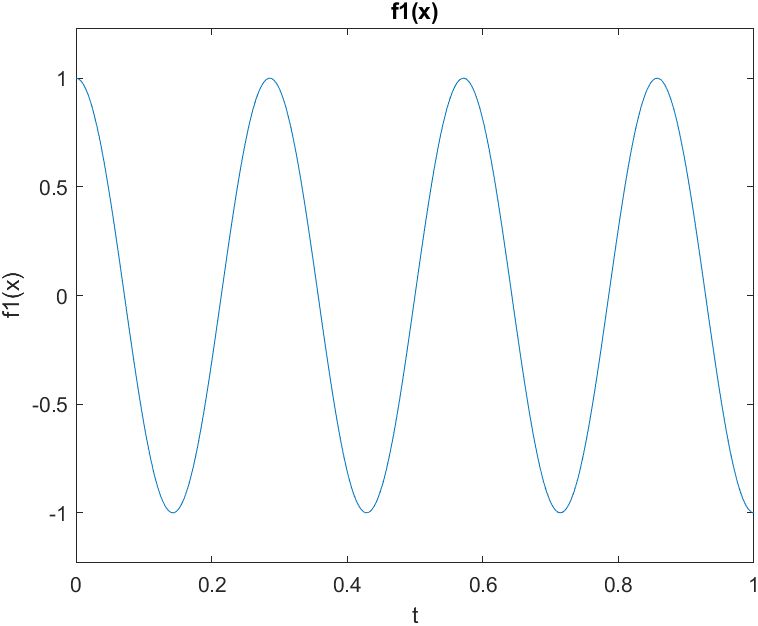
\includegraphics[width=0.4\textwidth]{f1-a.png}}%
    \qquad
    \subfloat[\centering f1(t) Fourier Transform (n=15)]{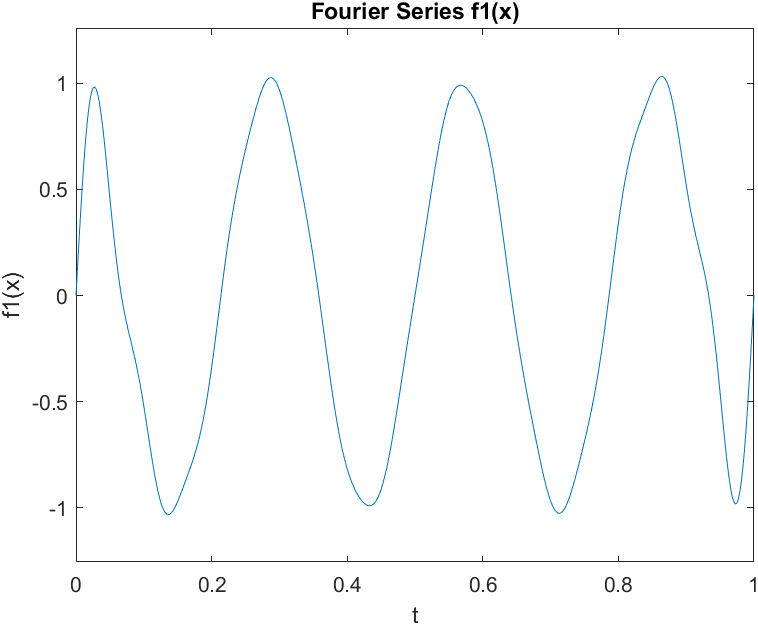
\includegraphics[width=0.4\textwidth]{f1-f.png}}%
    \caption{f1(t) compared to Fourier Series of f1(t).}
    \label{fig:f1-a}
\end{figure}




\subsubsection{B:}
\begin{equation*}
	\left.  a_{0}=\int_{0}^{1} 2x-1 dx = x(x-1) \right |_{0}^{1} =0
\end{equation*}
\begin{equation*}
	a_{n}=2 \int_{0}^{1} (2x-1)\cos(2\pi nx) dx = \frac{2\sin(\pi n)(\pi n \cos(\pi n)-\sin(\pi n))}{(\pi n )^2}
\end{equation*}
\begin{equation*}
	b_{n}=2 \int_{0}^{1} \cos(7 \pi x)\sin(2\pi nx) dx = \frac{2\cos(\pi n)(\sin(\pi n)-\pi n \cos(\pi n))}{(\pi n )^2}
\end{equation*}

\begin{equation*}
	\implies  f_2(t)=\sum_{n=1}^{\infty} [ \frac{2\sin(\pi n)(\pi n \cos(\pi n)-\sin(\pi n))}{(\pi n )^2}\cos(2\pi nt) +\frac{2\cos(\pi n)(\sin(\pi n)-\pi n \cos(\pi n))}{(\pi n )^2} \sin(2\pi)], 0 \leq t \leq 1
\end{equation*}
\begin{figure}
    \centering
    \subfloat[\centering f2(t) ]{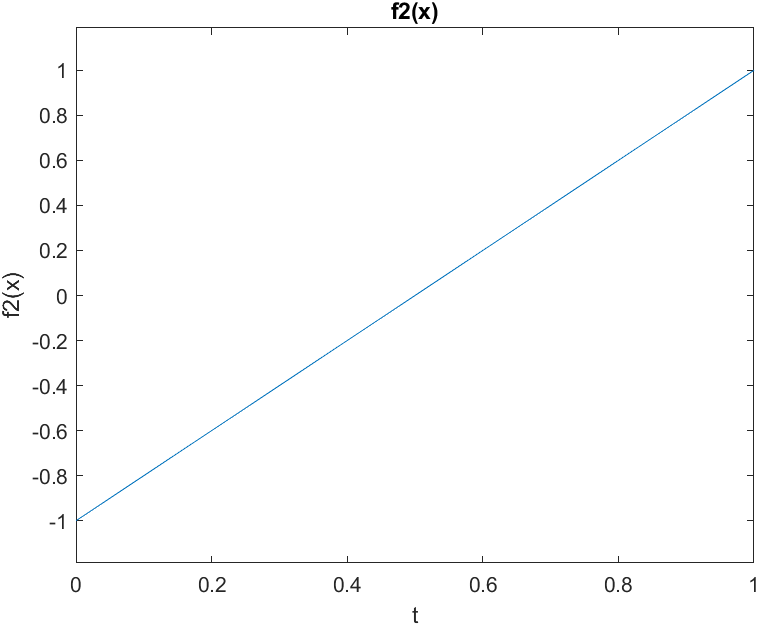
\includegraphics[width=0.4\textwidth]{f2-a.png}}%
    \qquad
    \subfloat[\centering f2(t) Fourier Transform (n=15) ]{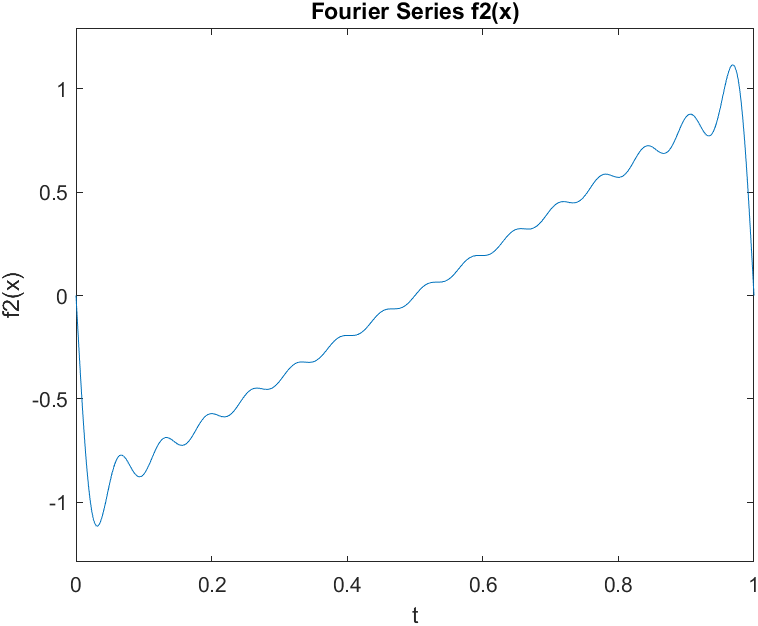
\includegraphics[width=0.4\textwidth]{f2-f.png}}%
    \caption{f2(t) compared to Fourier Series of f2(t).}
    \label{fig:f2-a}
\end{figure}

\subsubsection{C:}
\begin{equation*}
	 a_{0}=\frac{1}{2}\int_{0}^{1} dx -\frac{1}{2}\int_{1}^{2} dx  =0 
\end{equation*}

\begin{equation*}
	a_{n}= \int_{0}^{1}\cos(\pi nx) dx -\int_{1}^{2}\cos(\pi nx) dx= \frac{2\sin(\pi n)-\sin(2\pi n)}{\pi n}
\end{equation*}

\begin{equation*}
	b_{n}=\int_{0}^{1} \sin(\pi nx) dx -\int_{1}^{2} \sin(\pi nx) dx= \frac{1-2\cos(\pi n)+\cos(2\pi n)}{\pi n}
\end{equation*}
\begin{equation*}
	\implies  f_3(t)=\sum_{n=1}^{\infty} [ \frac{2\sin(\pi n)-\sin(2\pi n)}{\pi n}\cos(\pi nt)+\frac{1-2\cos(\pi n)+\cos(2\pi n)}{\pi n} \sin(\pi nt)], 0 \leq t \leq 2
\end{equation*}
\begin{figure}
    \centering
    \subfloat[\centering f3(t) ]{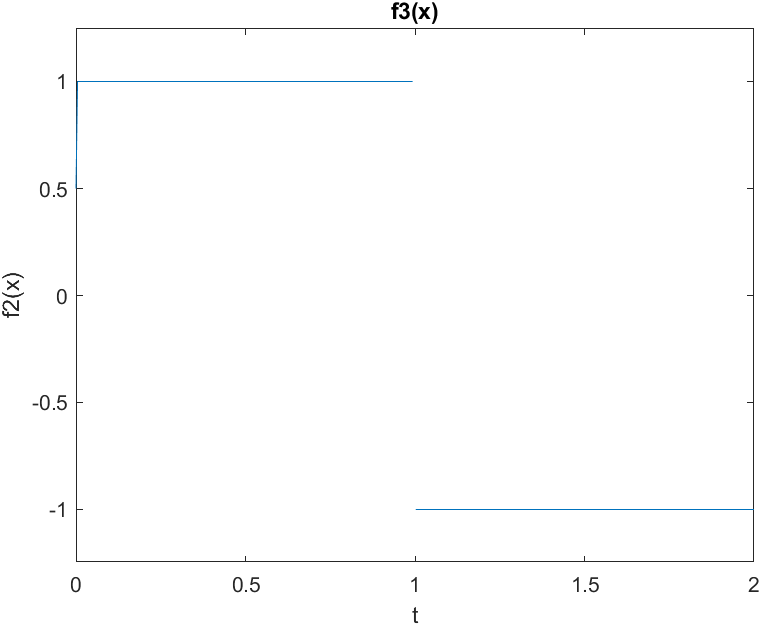
\includegraphics[width=0.4\textwidth]{f3-a.png}}%
    \qquad
    \subfloat[\centering f3(t) Fourier Transform (n=15)]{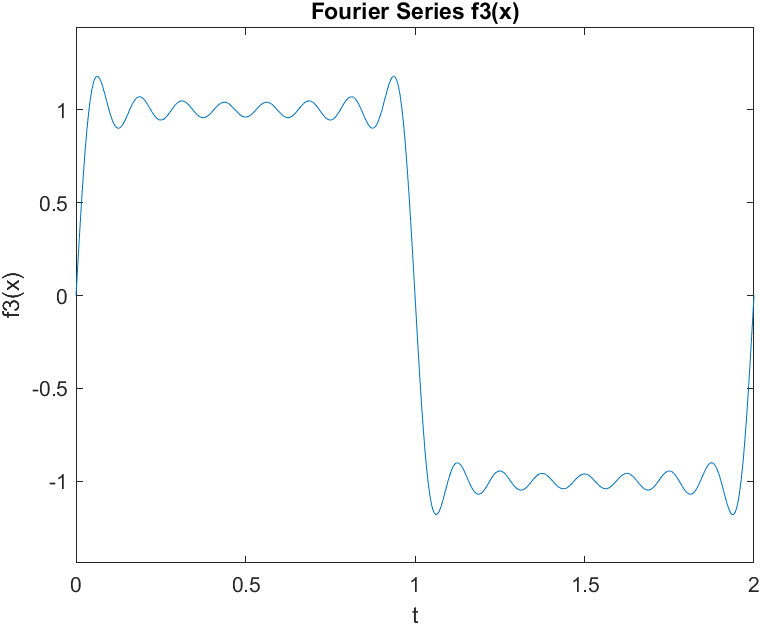
\includegraphics[width=0.4\textwidth]{f3-f.png}}%
    \caption{f3(t) compared to Fourier Series of f3(t).}
    \label{fig:f3-a}
\end{figure}

\subsection{Applications of Fourier Series: The displacement of a string}
A Fourier series can be used to determine the displacement of length $l=1$ if $u(x,0)=sin(\pi x)$ and $u_t(x,0)=0, 0 \leq x \leq 1$. Assuming that $u(0,t)=u(l,t)=0$  $\forall$  $t \ge 0$, meaning the ends of the string are held fixed, and that $c=2$.

\subsubsection{Initial Cases}
To solve $X''+\sigma X = 0$, three cases of sigma ($\sigma < 0, \sigma = 0, \sigma >0$) must be considered in addition to satisfying the boundary conditions $u(0,t)=u(l,t)=0$. Only $\sigma > 0$ is possible in this case [1].  This assumption combined with $\lambda^2 = \sigma$ implies the solutions are
\begin{equation*}
	X(x)=Acos(\lambda x)+B\sin(\lambda x).
\end{equation*}
For the initial condition of $u(0,t)=0$ to be satisfied, $X(0)=0 \implies A=0$. Additionally, $u(l,t)=0 \implies \sin(\lambda l) = 0 \implies \lambda l = n\pi, n \in \mathbb{Z}^{+}$. This means $\lambda_n = \frac{n\pi}{l}$ and $\sigma_n \frac{n^2 \pi ^2}{l^2}$. Therefore, for each positive integer
\begin{equation*}
	X_n(x)=B_n \sin(\frac{n\pi}{l} x)
\end{equation*}
\subsubsection{The Differential Equation}
Each $\sigma_n$ requires the solution of $T''_n(t) +c^2 \sigma_n T_n(t)=0$. The characteristic equation for this differential equation is
\begin{equation*}
r^2+c^2 \sigma_n=0,
\end{equation*}\begin{equation*}
\implies r:= \pm \omega_n i \pm c\sqrt{\sigma_n}i, \forall n \ge 1.
\end{equation*}
Notice: the components of $T_n(t)$ are periodic, implying the oscillation of the string is also periodic.

\subsubsection{General solution of the wave equation}
The general solution of the wave equation is given by a linear combination of solutions $X_n(x)T_n(t):$

\begin{equation*}
	u(x,t)=\sum_{n=1}^{\infty}[A_n \sin(\frac{n\pi}{l}x)\cos(\omega_n t)+B_n\sin(\frac{n\pi}{l}x)\sin(\omega_n t)]
\end{equation*}
\begin{equation*}
\implies  u(x,0)= \sum_{n=1}^{\infty} A_n \sin(\frac{n\pi}{l}x)
\end{equation*}
\begin{equation*}
\implies  u_t(x,0)= \sum_{n=1}^{\infty} \omega_n B_n \sin(\frac{n\pi}{l}x)
\end{equation*}Both  of the two equations above represent a Fourier sine series.


\subsubsection{Particular Solution}
$u(x,0)$  and $u_t(x,0)$ must be considered as odd functions with a domain of [$-l,l$] by reflection to determine the values of $A_n$ and $B_n$. For example $u(-x,0) = -u(x,0), 0 < x < l$. Hence, there will not be any constant or cosine terms in the Fourier series because this is an odd function. Therefore, the coefficients $A_n$ will be the Fourier coefficients of the reflected function. Using a symmetry argument, $A_n$ is 

\begin{equation*}
A_n=\frac{2}{l} \int_0^l u(x,0)\sin(\frac{n\pi}{l}x)dx.
\end{equation*}
Given the initial values

\begin{equation*}
A_n=2 \int_0^1  \sin(\pi x)\sin(n\pi x) dx =\frac{2\sin(n\pi)}{\pi -\pi n^2}.
\end{equation*}

Similarly, an an analogous expression for $B_n$ can be derived
\begin{equation*}
B_n = \frac{2}{\omega_n l} \int_0^l u_t(x,0)\sin(\frac{n\pi}{l}x)dx.
\end{equation*}Given the initial values

\begin{equation*}
B_n=0.
\end{equation*}

Substituting these in the original equation shows

\begin{equation*}
	u(x,t)=\sum_{n=1}^{\infty}[\frac{2\sin(n\pi)}{\pi -\pi n^2} \sin(n\pi x)\cos(2n\pi t)]
\end{equation*}
Note: given the boundary and initial conditions, the wave equation has a unique solution [2], [3].

\begin{figure}
    \centering
    \subfloat[\centering u(x,1) (n=1)]{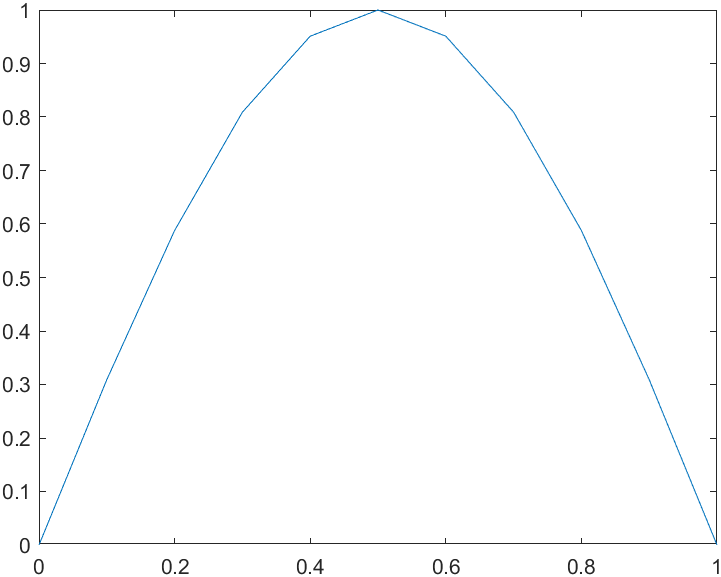
\includegraphics[width=4cm]{oneDwave0.png}}%
    \qquad
    \subfloat[\centering u(x,1.5) (n=1)]{\includegraphics[width=4cm]{oneDwave1.png}}%
    \caption{f1(t) compared to Fourier Series of f1(t).}
    \label{fig:f1-a}
\end{figure}

\subsubsection{Animation:}

\includegraphics{1D-wave.gif}
Note: Please load PDF in adobe acrobat reader dc.





\section{References}

[1]W. E. Boyce and R. C. DiPrima, Elementary differential equations and boundary value problems, 7th ed. New York: Wiley, 2001.
\newline
[2]Das, K. P. Integral Transforms and Their Applications. Alpha Science International Ltd., 2019. 
\newline
[3][Prof. Arthur Mattuck]. [Differential Equations]. [Fall 2011]. Massachusetts Institute of Technology: MIT OpenCouseWare, https://ocw.mit.edu/. License: Creative Commons BY-NC-SA.


\section{MATLAB Code}

\begin{listing}[h]
\inputminted{matlab}{FourierSeries.m}
\caption{Fourier Series code to plot the functions in (2.3).}
\label{listing:Fourier-Code}
\end{listing}

\begin{listing}[h1]
\inputminted{matlab}{OneDWave.m}
\caption{1D Wave code  to plot the functions in (2.4).}
\label{listing:Fourier-Code}
\end{listing}



\end{appendices}

\end{document}
